\subsection{Adaptation of task clustering}\label{s:SchedHyperflow:Agglomeration}

%% można opisać phase-opt jako vertical clustering, ale odrzucić


%% this chapter zamiast work?
An expansion of the scheduling problem described in this work is task clustering.
In Hyperflow, \emph{job agglomeration} is managed through the use of \emph{functions} as it is mentioned in section \ref{s:ProblemDomain:Hyperflow}.
However, the current approach with a single task buffer has a few limitations that are not compatible with the presented scheduling solution.
% The states  are shown in \todo{\\cref{}}.

% w Hyperflow Jest ścisle zwiazany z implementacja w wms.
% Dokonano modyfikacji w celu przebadania wersji ze schedulingiem.


% Obecna wersja (diagram?) -> Pliki konfiguracyjne. -> jeden bufor -> ustalony rozmiar bufora -> horyzontalnie


% Adaptowana (diagram stanów) -> automagiczne -> bufor per cpu -> maksymalna objętość -> minimalizacja ilości tworzonych kontenerów -> horyzontalnie -> istnieje możliwość wertykalnej (phase opt), ale kontenery mogą być rózne, więc lepiej nie 


% Since the experiment is being run with Hyperflow engine in Kubernetes cluster, it has been decided not to change the solution entirely.
To adopt the idea of clustering into the scheduling concept, the number of active buffers used in the process has been adjusted to the number of available computing units.
This allows to agglomerate jobs within a preplanned task sequence associated with a given processor.
The diagram in \cref{fig:solution:k8s-states-buffer} presents the states of an modified Hyperflow buffering function for Kubernetes jobs. 

%%% diagram stanów

%%%%
\begin{figure}[H]
\centering
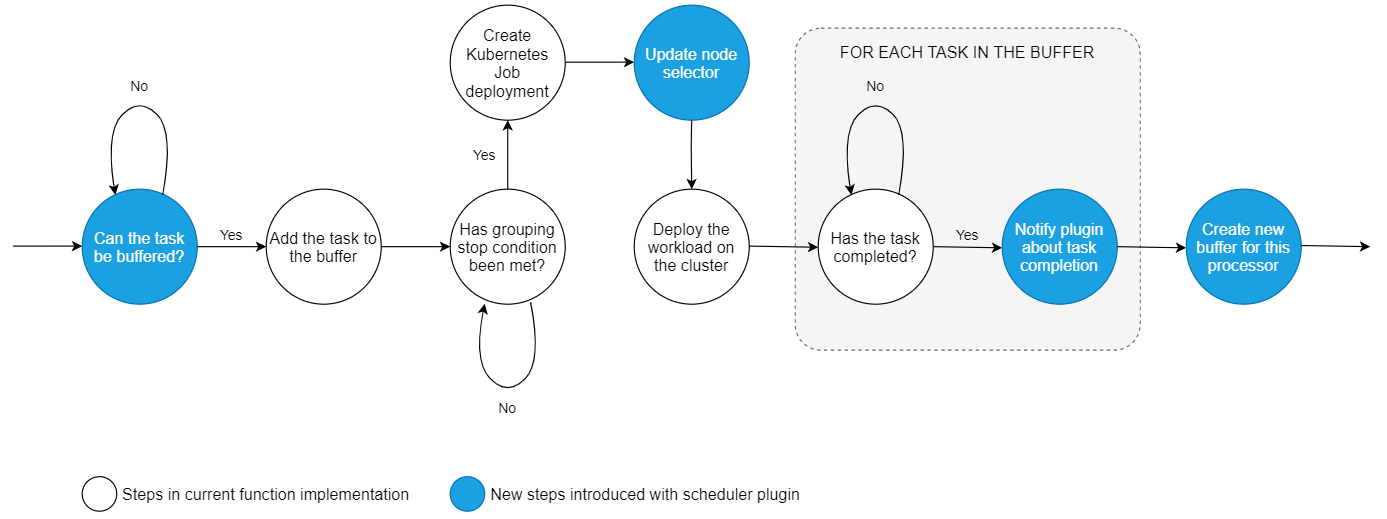
\includegraphics[width=1\linewidth]{figures/4-2-K8sBufferFunction.png}
\caption[Adjusted Hyperflow function for scheduling clusterized workloads]{States of an adjusted function for scheduling clustered tasks as Kubernetes jobs.}

% \medskip
% \begin{minipage}{0.67\textwidth}
% {\footnotesize The diagram presents states in a processor specific context a task specific buffering flow.
% diagram contains states eac permissions from the scheduler plugin are a mechanism to ensure the correct order of execution for a single specific computing unit. \par}
% \end{minipage}

\label{fig:solution:k8s-states-buffer}
\end{figure}
%%%%

% With these adjustments, a conceptual behaviour has not changed.

The task clusterization approach is still horizontal, although it happens only in the context of a single computing unit.
This means the tasks still are being buffered only with the other ones that run the operation.
In the current solution, the buffers require a configuration for their maximum task capacity.
It is set to prevent the possible imbalanced resource consumption that could happen when a majority of tasks from the same horizontal level are grouped into a single buffer.
Utilization of all available resources, or at least the possibility of their inclusion during the execution process, are guaranteed by the schedule.
Therefore, there is no longer a need to setup limits on the maximum buffer size.
This could help to reduce the overhead for workload containerization during the workflow execution, which will be inquired during the analysis of experimental results.
To better comprehend the differences between the two, the example traces from \cref{fig:solution:agglo:traces} present a workflow execution with both approaches.




%%%%
\begin{figure}[H]
\begin{subfigure}{1\textwidth}
\centering
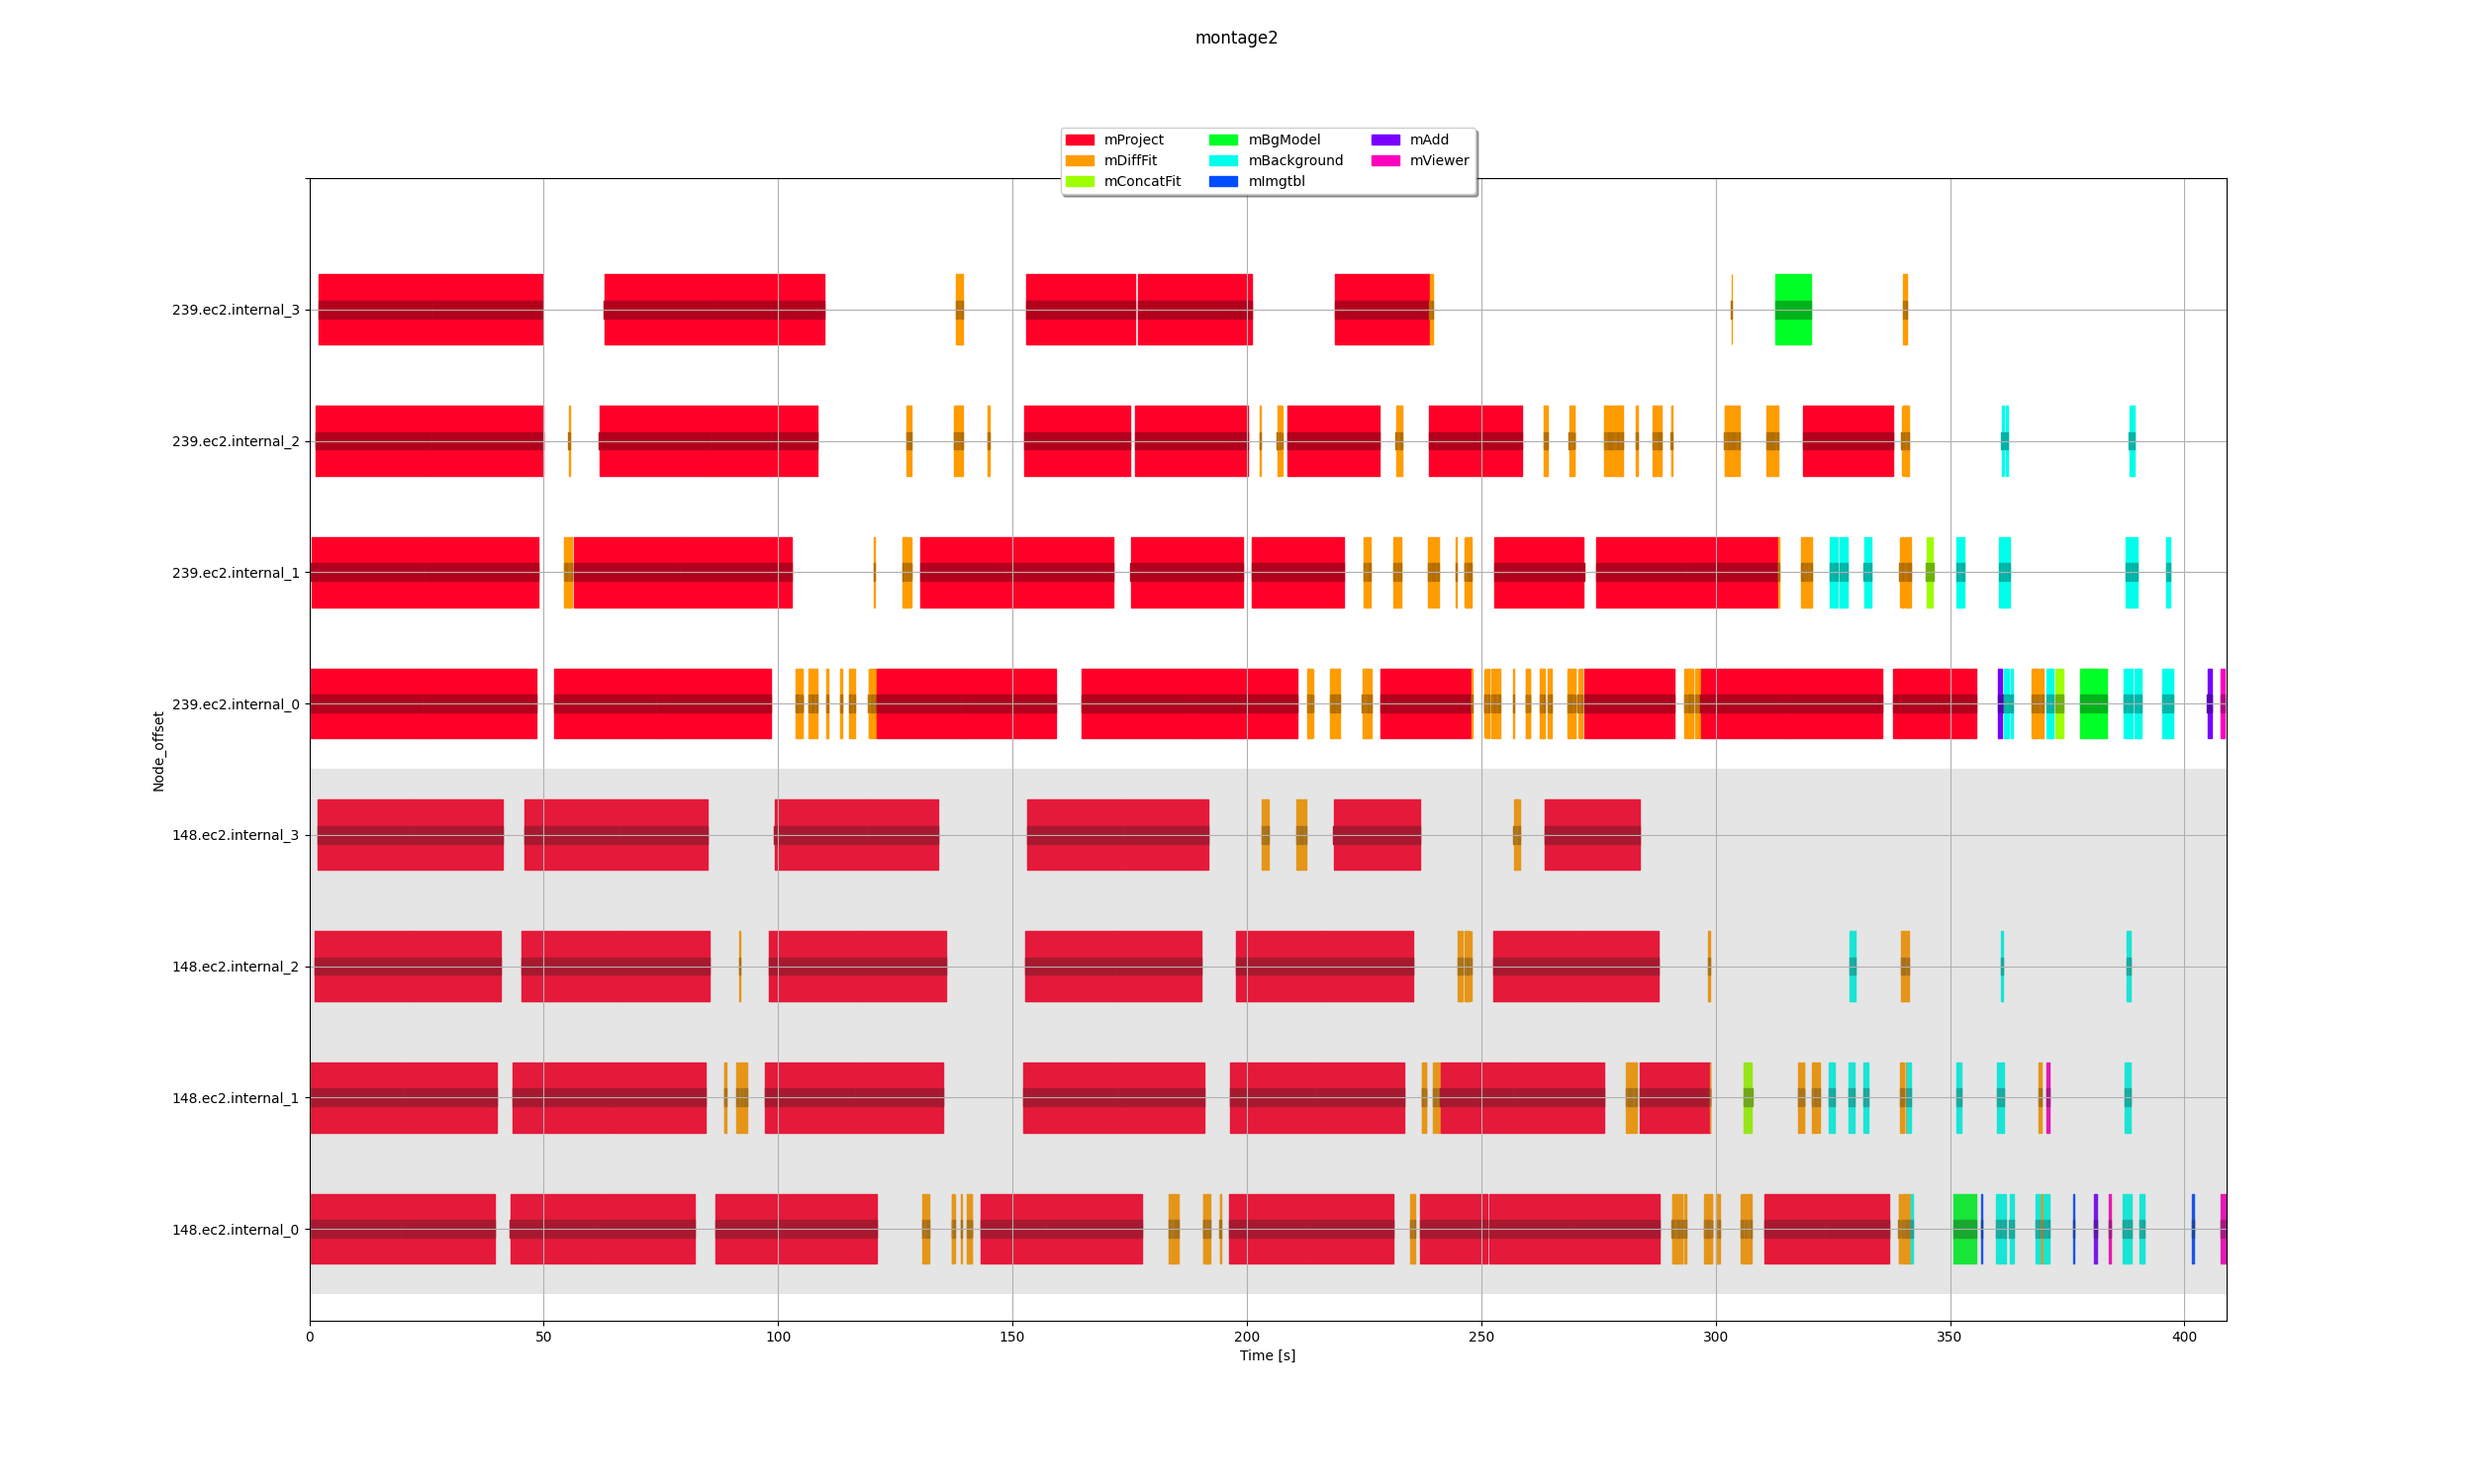
\includegraphics[width=1\linewidth]{figures/4-2-AggloEMPTY.png}
\caption[Agglo EMPTY]{Standard job agglomeration in Hyperflow.}
\label{fig:solution:agglo:empty}
\end{subfigure}
\begin{subfigure}{1\textwidth}
\centering
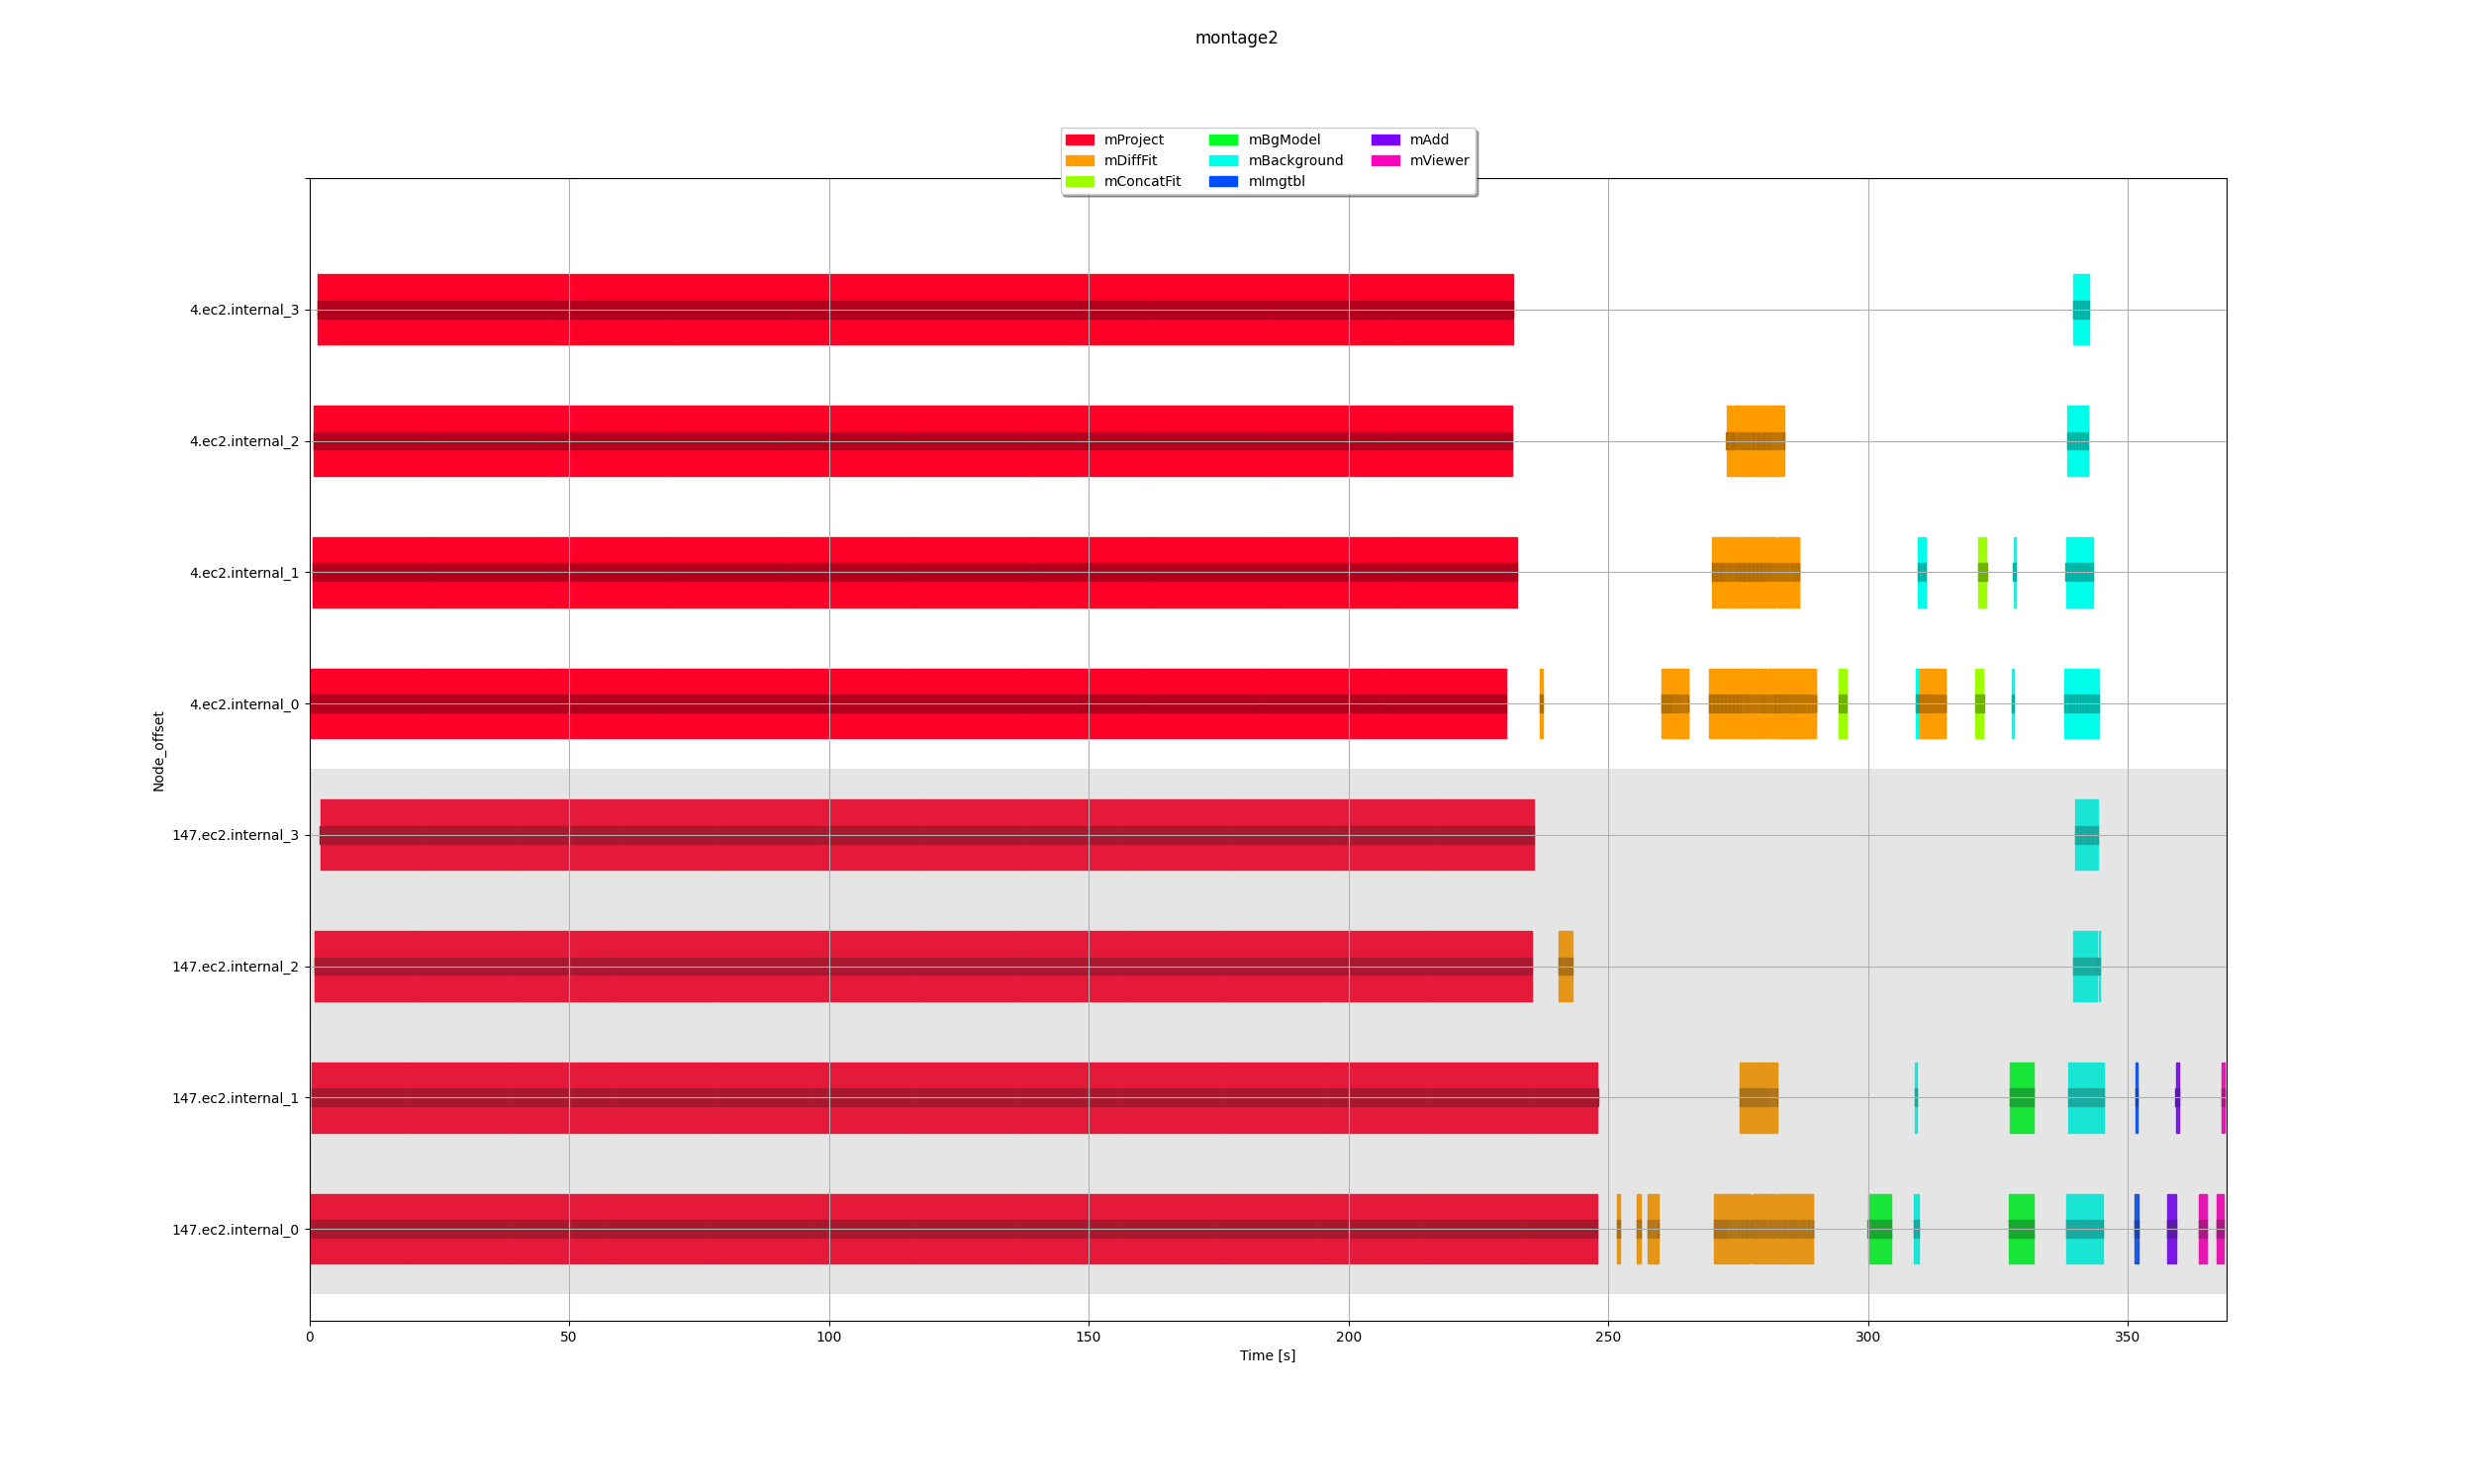
\includegraphics[width=1\linewidth]{figures/4-2-AggloHEFT.png}
\caption[Agglo HEFT]{Modified agglomeration after scheduling with HEFT.}
\label{fig:solution:agglo:heft}
\end{subfigure}
\centering

\caption[Differences in execution traces with task clustering]{Comparison of execution traces with different task clustering approaches. Having no limitations on maximum buffer sizes allows creation of a single container with longer lifespan instead of multiple ones for a short periods of time.}

% \medskip
% \begin{minipage}{0.75\textwidth}
% {\footnotesize Having no limitations on maximum buffer sizes allows creation of a single container with longer lifespan instead of multiple ones for a short periods of time. \par}
% \end{minipage}

\label{fig:solution:agglo:traces}
\end{figure}
%%%%